% Latex template: mahmoud.s.fahmy@students.kasralainy.edu.eg
% For more details: https://www.sharelatex.com/learn/Beamer

\documentclass[aspectratio=1610]{beamer}					% Document class

\setbeamertemplate{footline}[text line]{%
  \parbox{\linewidth}{\vspace*{-8pt}The relationship between chromatin structure and transcriptional dynamics \hfill\insertshortauthor\hfill\insertpagenumber}}
\setbeamertemplate{navigation symbols}{}

\usepackage[english]{babel}				% Set language
\usepackage[utf8x]{inputenc}			% Set encoding

\mode<presentation>						% Set options
{
  \usetheme{default}					% Set theme
  \usecolortheme{default} 				% Set colors
  \usefonttheme{default}  				% Set font theme
  \setbeamertemplate{caption}[numbered]	% Set caption to be numbered
}

% Uncomment this to have the outline at the beginning of each section highlighted.
%\AtBeginSection[]
%{
%  \begin{frame}{Outline}
%    \tableofcontents[currentsection]
%  \end{frame}
\usepackage{graphicx}					% For including figures
\usepackage{booktabs}					% For table rules
\usepackage{hyperref}	
\usepackage{tikz-network}				% For cross-referencing
\usepackage[absolute,overlay]{textpos}
\usepackage{bm}
\usepackage[font=small,labelfont=bf]{caption}				% For cross-referencing

\title{The relationship between chromatin structure and transcriptional dynamics}	% Presentation title
\author{Clayton W. Seitz}								% Presentation author
\date{\today}									% Today's date	

\begin{document}

% Title page
% This page includes the informations defined earlier including title, author/s, affiliation/s and the date
\begin{frame}
  \titlepage
\end{frame}


% The following is the most frequently used slide types in beamer
% The slide structure is as follows:
%
%\begin{frame}{<slide-title>}
%	<content>
%\end{frame}


\begin{frame}{Summary}
\begin{itemize}
\item Preliminary data for GBP5 and GAPDH co-staining
\item The relationship between chromatin structure and transcription dynamics
\end{itemize}
\end{frame}

\begin{frame}{RNA flow model for transcription dynamics}
\begin{figure}
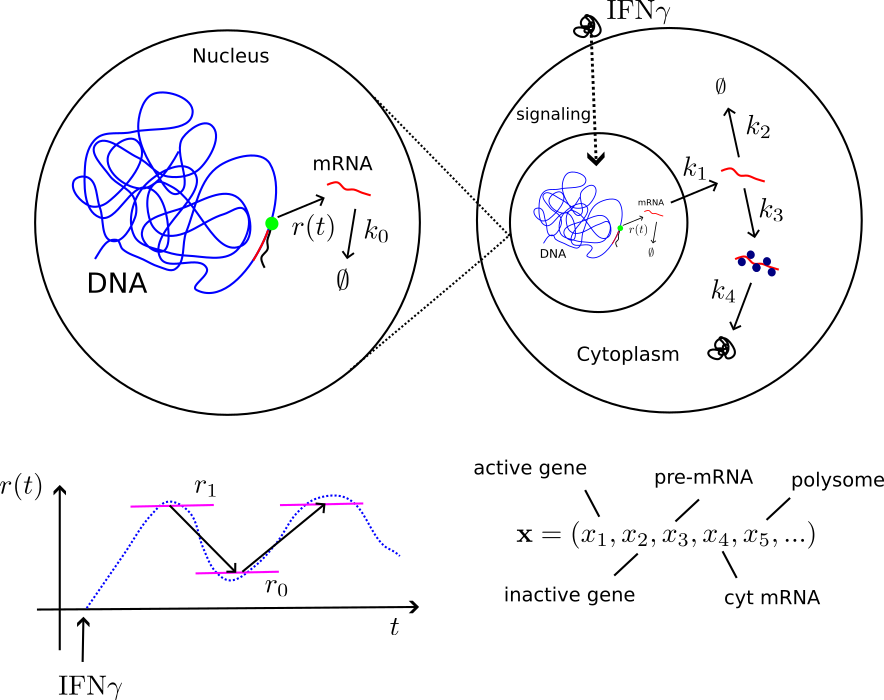
\includegraphics[width=10cm]{RNAFlow.png}
\end{figure}
\end{frame}

\begin{frame}{Rare HeLa cell GBP5 expression @ 24h after reinduction with IFN-$\gamma$}
\begin{figure}
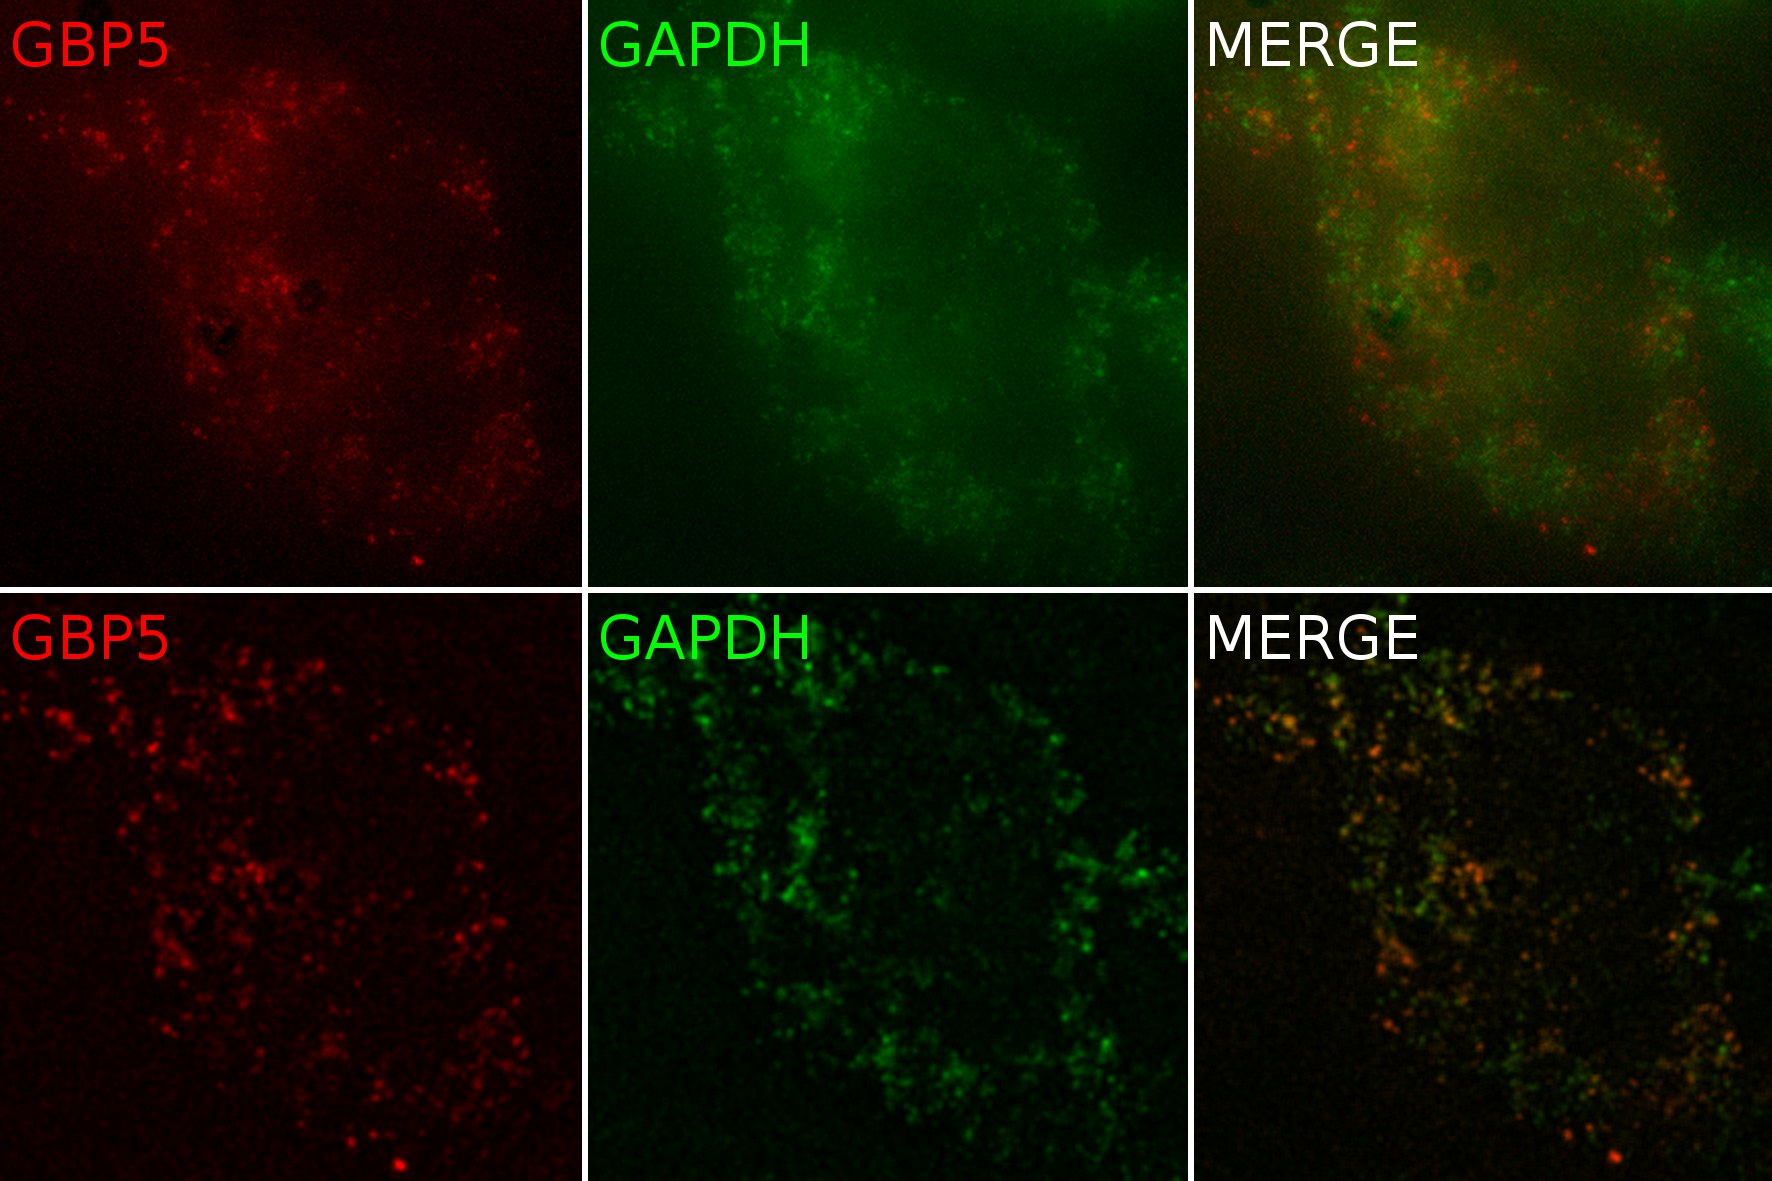
\includegraphics[width=12cm]{Stains.png}
\end{figure}
\end{frame}

\begin{frame}{Intensity histogram for rare GBP5 expression}
\begin{figure}
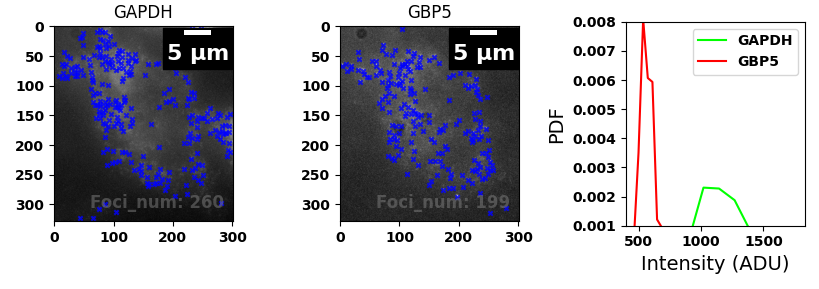
\includegraphics[width=14cm]{Detection.png}
\end{figure}
\begin{itemize}
\item \textcolor{red}{Very few ($\sim 1\%$)} reinduced cells express GBP5, but those that do express at high levels (relative to GAPDH)
\item Waiting on the control to determine if this effect is coupled to IFN-$\gamma$ 
\item RNA flow model may have no meaning (GBP5 transcription is non-ergodic)
\end{itemize}
\end{frame}

\begin{frame}{Sources of variability in the rate of gene expression}
\vspace{0.1in}
\begin{itemize}
\item Previous work suggests that IFN-$\gamma$ induces epigenetic changes at the GBP5 locus
\item If some cells get the epigenetic change and others dont, the model breaks down
\end{itemize}

\begin{figure}
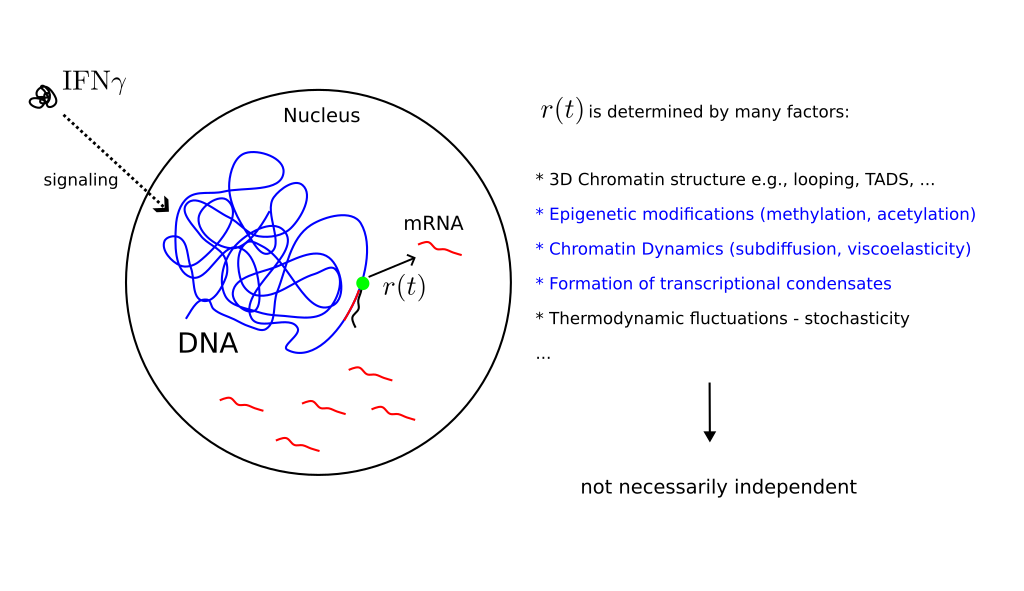
\includegraphics[width=13cm]{Sources.png}
\end{figure}
\end{frame}

\begin{frame}{}
Paper on epigenetic modifications to chromatin structure
\end{frame}

\end{document}